\section{实验设计}

本实验系统由四个主要模块组成:Hamming 编解码、交织与解交织、QPSK 调制解调以及加性高斯白噪声(AWGN)信道。这些模块协同工作,模拟实际通信系统中的信号处理与传输过程。

\subsection{Hamming 编解码}

在通信系统中,通过在信源中添加冗余信息,可以使信道传输后的结果具有一定的检错与纠错能力。本系统中采用 (7,4) Hamming信道编码,即将 4 位信息bit转换为7位编码bit,经过信道传输后纠错并转换回4位信息bit。具体原理表述如下:

设 $\bm{m}$ 为 $k$ 位信息bit矢量,定义生成矩阵 $G_{k\times n}=[I_{k\times k}; P_{k\times(n-k)}]$ 为单位矩阵 $I$ 与奇偶校验阵 $P$ 的组合,编码后的结果为 $\bm{x}=\bm{m}G=[\bm{m};\bm{m}P]$。记 $H^T=\begin{bmatrix}P\\I\end{bmatrix}$ 为校验矩阵,由于 $GH^T=\begin{bmatrix}I;P\end{bmatrix}\begin{bmatrix}P\\I\end{bmatrix}=P+P=0$,故合法码字一定满足 $\bm{x}H^T=0$。由于Hamming码的最小码距为3,故最多纠一位错,设通过信道后的bit串为 $\bm{y}=\bm{x}+\bm{e}$,其中 $\bm{e}$ 为长度为 $n$ 且最多只有一位为1的矢量,则校正子 $\bm{s}=\bm{y}H^T=\bm{x}H^T+\bm{e}H^T=\bm{e}H^T$ 为 $H^T$ 矩阵中的某一行,将校正子与 $H^T$ 比较即可得出错误bit位置,从而完成纠错。

\subsection{交织与解交织}

在通信系统中,由于无线信道的深衰落等原因,有可能使得系统中存在不可抗拒的连续突发错误,这使得一组码字中可能出现多于 1 位的错误,则 Hamming 码的纠错能力大大下降。为此,可在编码后引入一个交织器,典型的交织器让信息序列按行写入,按列读出,使得原本相邻的码元在时间上的距离最大化。如图 \ref{fig:interleave_model} 所示,交织矩阵的列数一般不小于分组码长,交织矩阵的行数不小于突发错最大长度。一个交织块的长度为交织矩阵的列数乘行数,略小于交织延时和解交织延时。交织块总长度应为整数个编码块长度,以避免同一个编码块分到前后两个交织块引起过大延时。

\begin{figure}[ht]
    \centering
    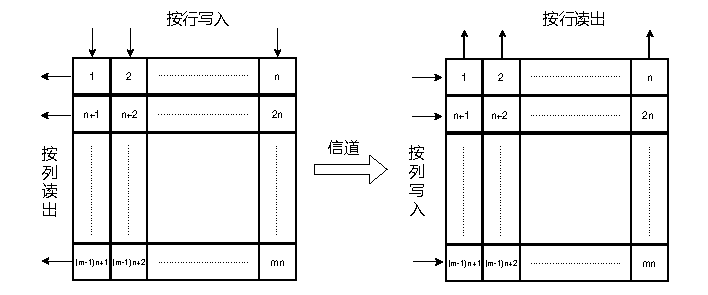
\includegraphics[width=.8\textwidth]{static/interleave_model.pdf}
    \caption{交织与解交织过程}
    \label{fig:interleave_model}
\end{figure}

在本次实验中,我们取交织矩阵的列数等于 Hamming 码长 $n=7$,交织矩阵的行数取 $m=4$,交织块的长度 $mn=28$. 

\subsection{QPSK 调制解调}

在现代数字通信系统中,QPSK(Quadrature Phase Shift Keying,正交相位调制)是一种高效的调制方式,它通过在同一时间内传输两个比特来实现高数据传输率。如图 \ref{fig:qpsk_model} 所示,QPSK 调制器将输入的二进制数据分成两部分,每部分表示一个信号的相位,分别控制正交的两个载波(I路和Q路)。这种方式可以有效利用带宽,同时保持较高的抗干扰能力。

\begin{figure}[ht]
    \centering
    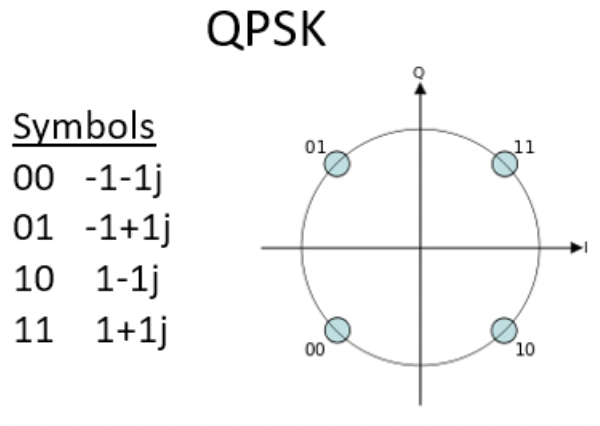
\includegraphics[width=.3\textwidth]{static/qpsk_model.png}
    \caption{QPSK 调制解调模型}
    \label{fig:qpsk_model}
\end{figure}

QPSK 调制与解调过程包括以下几个步骤:

\begin{itemize} 
    \item 调制过程:输入的数据每两位作为一个信号符号,映射到四个不同的相位上,通常是 $0^\circ$,$90^\circ$,$180^\circ$ 和 $270^\circ$,分别对应不同的比特组合。
    \item 解调过程:接收端根据信号的相位变化来恢复发送的比特流。通过比较接收到的信号与阈值,判断其属于哪个相位,并输出对应的比特组合。
\end{itemize}





\subsection{AWGN 信道模型}

AWGN(Additive White Gaussian Noise,加性白噪声)信道模型广泛应用于无线通信领域,用于模拟理想情况下的噪声影响。在此信道模型中,噪声是加性、均匀分布的,且具有高斯分布特性。在本实验中,AWGN 信道的模拟过程分为两个步骤:首先,通过 LFSR(线性反馈移位寄存器)生成伪随机数序列;然后,利用 Box-Muller 变换将这些伪随机数转换为服从高斯分布的随机数,最终将这些噪声加到信号中,模拟实际通信中的噪声干扰。

\subsubsection{LFSR}

为了产生 Gaussian 白噪声,首先需要生成均匀分布的伪随机数序列。本实验中,我们采用线性反馈移位寄存器(LFSR),通过移位寄存器和特定的反馈函数来生成这些随机数。

图 \ref{fig:lfsr_model} 展示了一个 16 位 Fibonacci LFSR。其采用的特征多项式为 $X^{16} + X^{14} + X^{13} + X^{11} + 1$。该多项式确保了生成的随机序列的周期最大(65535,不包括全零状态),以有效地模拟随机性。移位寄存器逐位输出随机序列的每一位,同时通过反馈机制决定下一个状态。这一过程不断重复,直到达到最大周期。例如,图中的状态为 0xACE1 (十六进制) ,下一个状态是 0x5670.

\begin{figure}[ht]
    \centering
    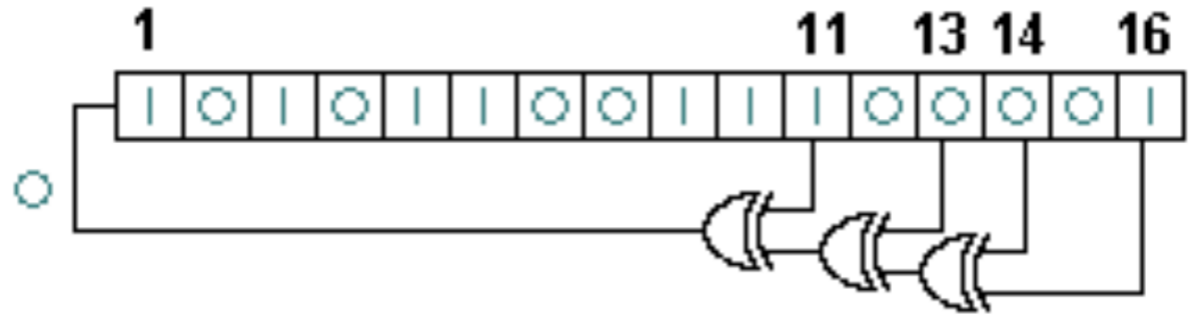
\includegraphics[width=.6\textwidth]{static/lfsr_model.png}
    \caption{一个 16-位 Fibonacci LFSR}
    \label{fig:lfsr_model}
\end{figure}

\subsubsection{Box-Muller}

Box-Muller 变换是一种用于从均匀分布的随机数生成高斯分布随机数的方法。在本实验中,我们首先生成两个均匀分布的随机数 $U_1, U_2 \sim U(0, 1)$,然后通过以下公式将其转换为符合标准正态分布的随机数:

$$
\begin{aligned}
X = \sqrt{-2\ln U_1} \cos(2\pi U_2) \\
Y = \sqrt{-2\ln U_1} \sin(2\pi U_2)
\end{aligned}
$$

其中,$X$ 和 $Y$ 分别为符合标准正态分布的随机变量。
